%% document class
\documentclass[10pt]{beamer}
%%theme
\usetheme[hideothersubsections,width=2cm]{Berkeley}
%% page settings
\usepackage{xcolor}
%%\usenavigationsymbolstemplate{}
\usefonttheme{structureitalicserif}
%%\defbeamertemplate*{footline}{shadow theme}

%% packages
\usepackage{courier}
\usepackage{geometry}
\usepackage{graphicx}
\usepackage[scaled=0.9]{helvet}
\usepackage{multimedia}
\usepackage{media9}
\usepackage{mathptmx}
\usepackage{tikz}
\usepackage{xmpmulti}
\usepackage{eso-pic}

%%color settings
%%%%% Color Schema
\definecolor{grey_dark}{RGB}{38,50,56}
\definecolor{grey}{RGB}{33,150,243}
\definecolor{gray_dark}{RGB}{39,36,41}
\definecolor{white}{RGB}{255,255,255}
\definecolor{orangish}{RGB}{255, 117, 26}
\definecolor{nvidia}{RGB}{116, 183, 27}
\definecolor{grey_light}{RGB}{242, 242, 242}

%% theme settings
\setbeamercolor*{palette primary}{fg=white,bg=grey_dark} % upper part
\setbeamercolor*{palette secondary}{fg=grey_dark,bg=nvidia} % left part (background)
\setbeamercolor*{sidebar left}{fg=white,bg=grey_dark} % left part with links
\setbeamercolor*{palette sidebar primary}{fg=nvidia}
\setbeamercolor*{palette sidebar secondary}{fg=white}
\setbeamercolor*{block title}{fg=grey_dark,bg=nvidia}
\setbeamercolor*{block body}{fg=grey_dark,bg=grey_light}
\setbeamercolor{section in toc}{fg=grey_dark}
\setbeamercolor{section number projected}{bg=nvidia}
\setbeamercolor*{item}{fg=nvidia} % bullets
\setbeamerfont{section in sidebar}{size=\scriptsize}

%% new commands
%\input{settings/macros}
\addtobeamertemplate{frametitle}{\vskip+0.6ex}{}
\makeatletter
\beamer@headheight=2\baselineskip
\makeatother

%% slide numbers
\makeatletter
\setbeamertemplate{frametitle}{%
	\nointerlineskip%
	\vskip-\beamer@headheight%
	\vbox to \beamer@headheight{%
		\vfil
		\leftskip=-\beamer@leftmargin%
		\advance\leftskip by0.3cm%
		\rightskip=-\beamer@rightmargin%
		\advance\rightskip by0.3cm plus1fil%
		{\usebeamercolor[fg]{frametitle}
			\usebeamerfont{frametitle}\insertframetitle\hfill\insertframenumber\par}% added number
		{\usebeamercolor[fg]{framesubtitle}
			\usebeamerfont{framesubtitle}\insertframesubtitle\par}%
		\vbox{}%
		\vskip-1em%
		\vfil
	}%
}
\makeatother

%% Logo
\newcommand\AtPagemyUpperLeft[1]{\AtPageLowerLeft{%
\put(\LenToUnit{0.05\paperwidth},\LenToUnit{0.89\paperheight}){#1}}}
\AddToShipoutPictureFG{
	\AtPagemyUpperLeft{{
\includegraphics[width=0.8cm,keepaspectratio]{images/kgp_logo.png}}}
}%

\begin{document}
\author[\textbf{Group 9}]{Sourav Kumar Singh\\Gopal Krishna\\Subhankar Halder\\Sayan Khan\\}
\title[\textbf{Deep Learning}]{Deep Learning and its applications using \LaTeX}
\institute[JGEC]{Jalpaiguri Govt Engineering College}

%% Title Page
{ % all template changes are local to this group.
	\setbeamertemplate{navigation symbols}{}
	\begin{frame}[plain]
		\begin{tikzpicture}[remember picture,overlay]
		\node[at=(current page.center)] {
			\includegraphics[width=\paperwidth]{images/title_bg}
		};
		\end{tikzpicture}
	\end{frame} 
}

%% Contributors Page
\begingroup
\usebackgroundtemplate{%
	\tikz\node[opacity=0.3] {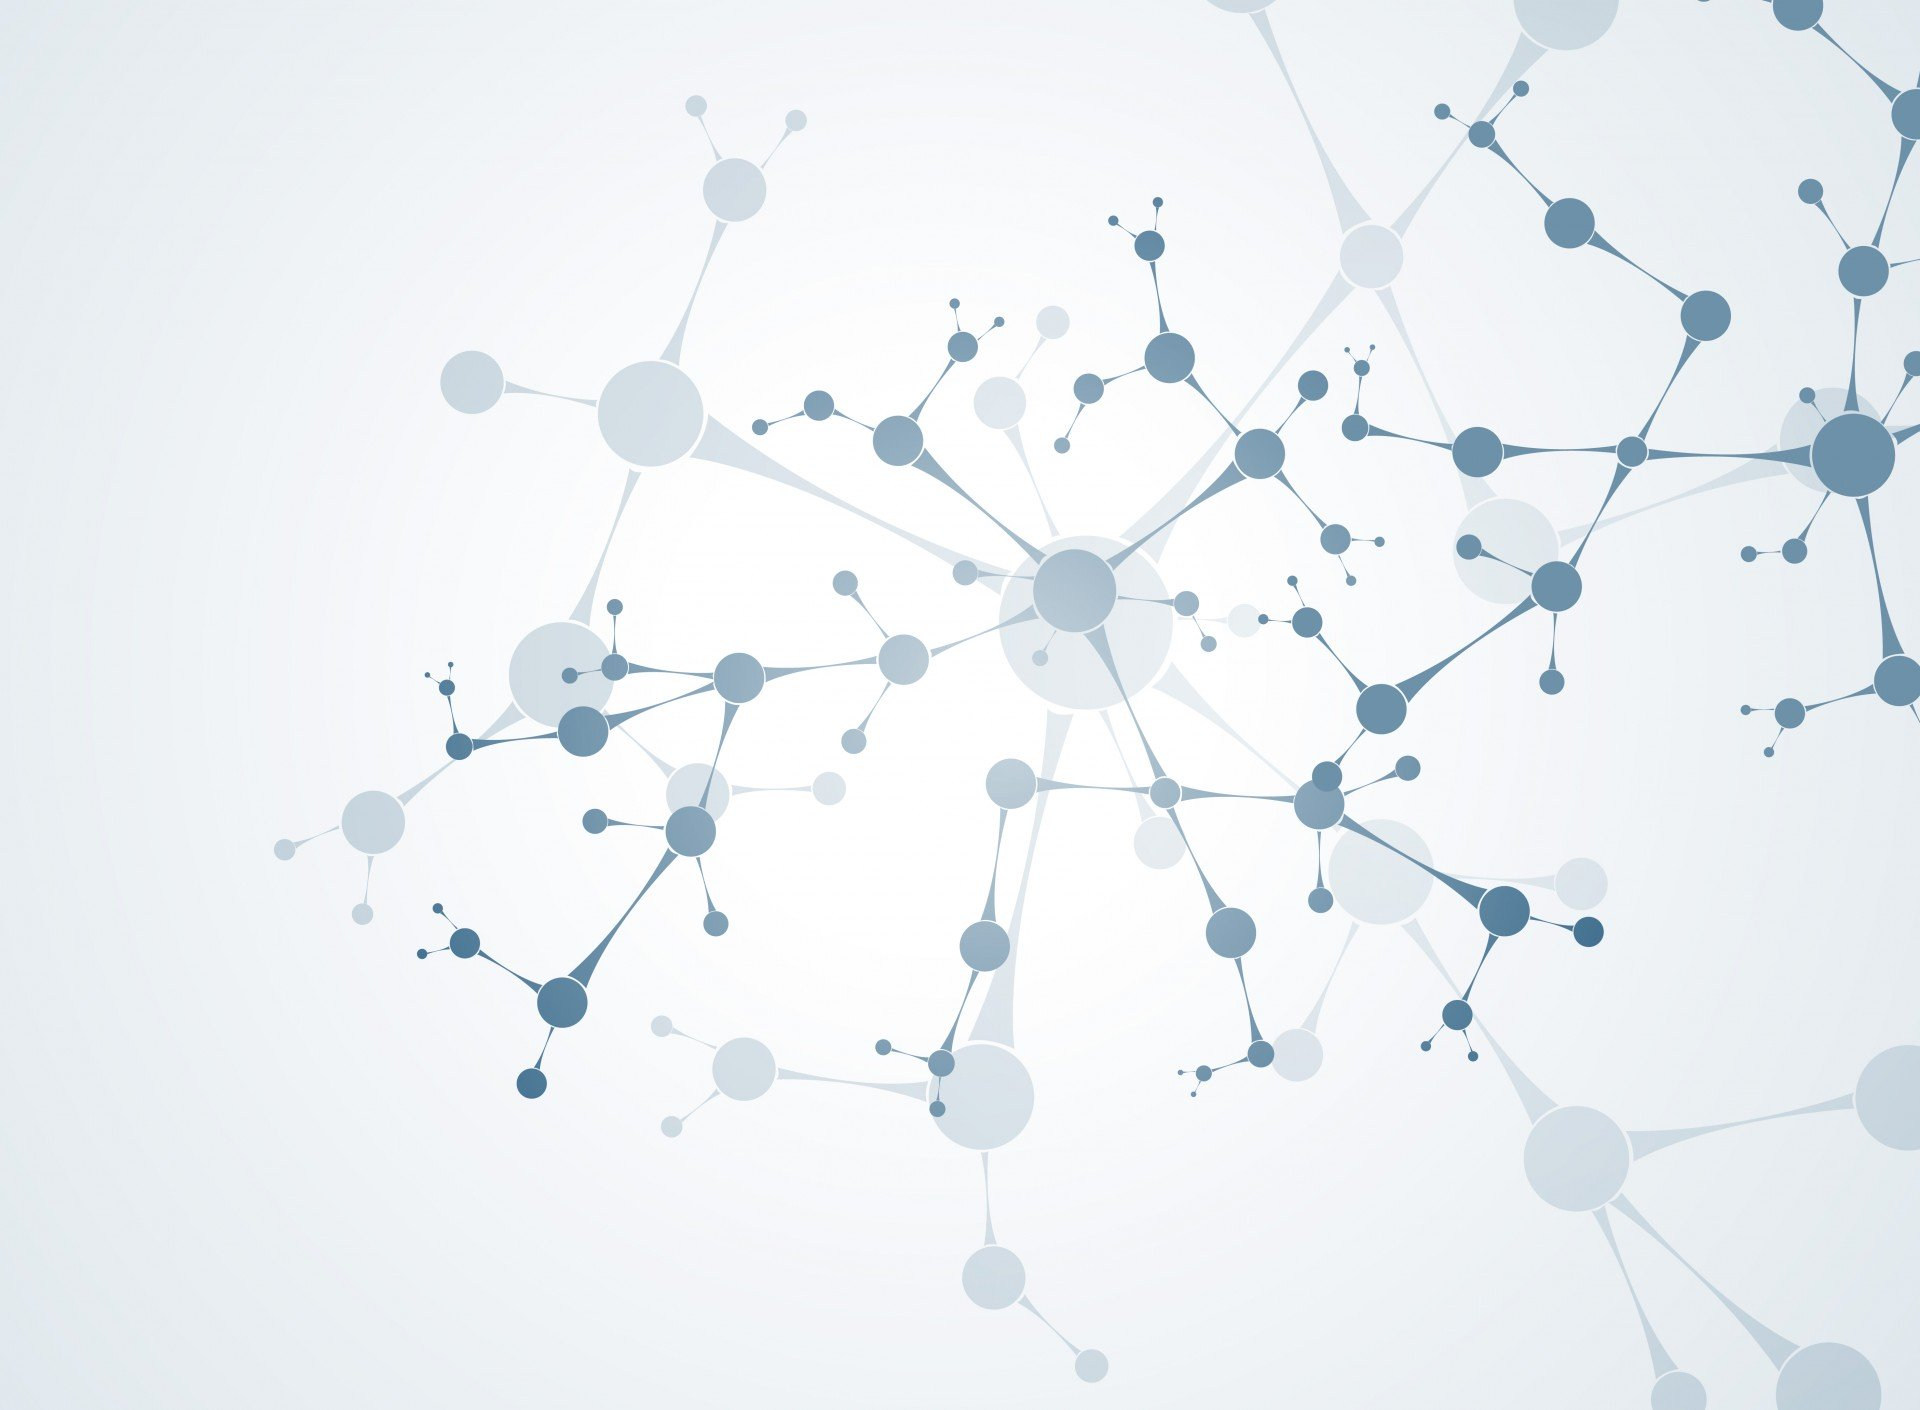
\includegraphics[height=\paperheight,width=\paperwidth]{images/bg-vec}}
	;}
	\begin{frame}[c]{Contributors}
		\begin{center}
			\Huge{Presented By:\\}
			\large{~\\Subhajit Barh\\}
		\end{center}
	\end{frame}
	%% contents
	\begin{frame}{Contents in Brief}
		%\tableofcontents
		\tableofcontents[hideallsubsections]
	\end{frame}
\endgroup

\begingroup
\usebackgroundtemplate{%
		\tikz\node[opacity=0.3] {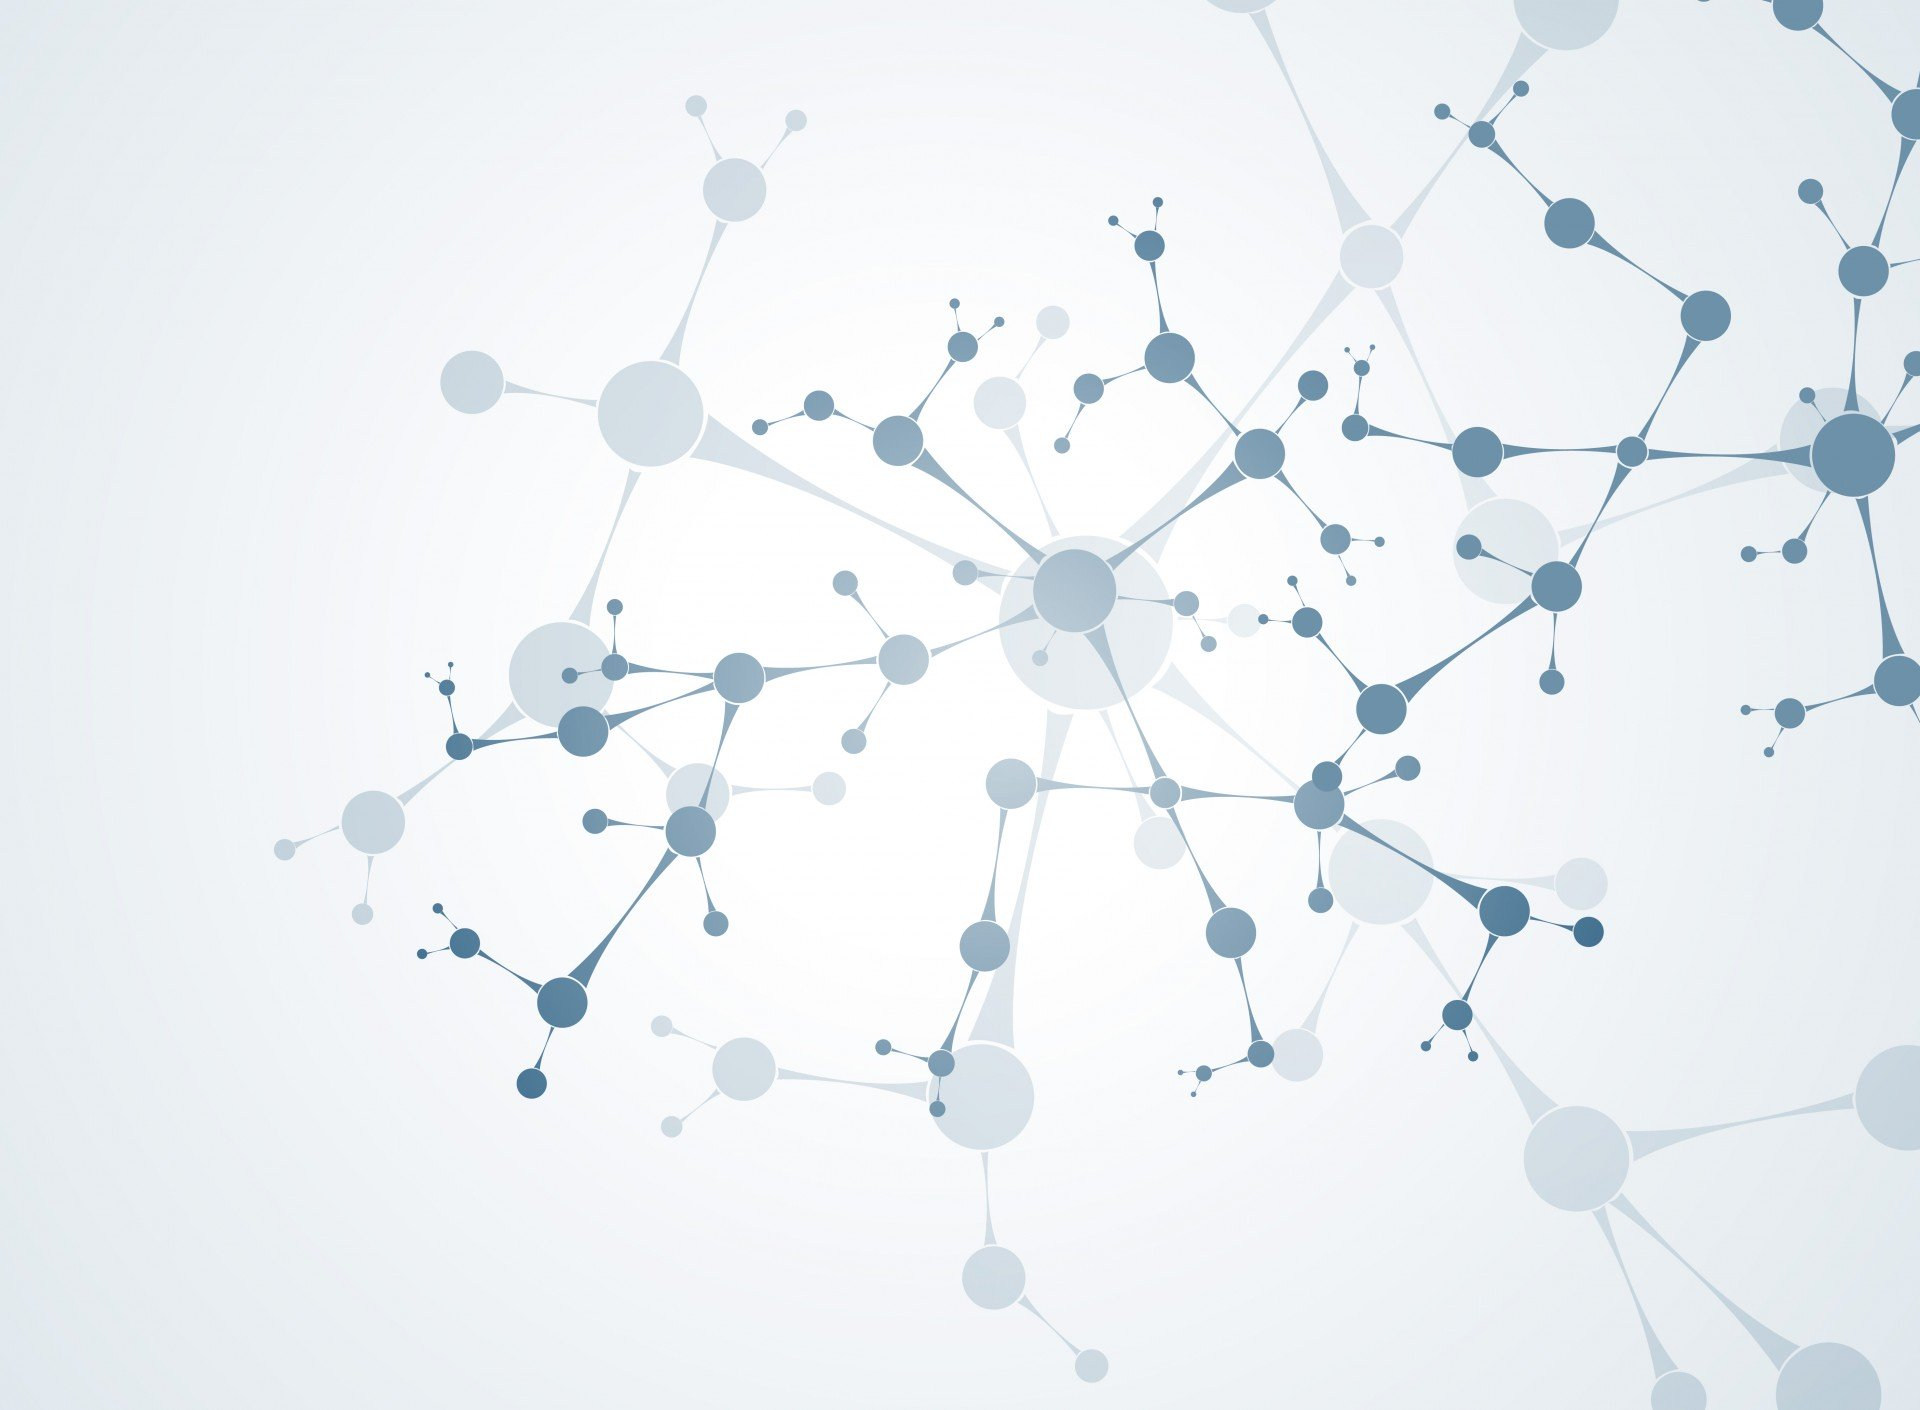
\includegraphics[height=\paperheight,width=\paperwidth]{images/bg-vec}}
		;}
	
	
	{ % all template changes are local to this group.
		\setbeamertemplate{navigation symbols}{}
		\begin{frame}[plain]
		\begin{tikzpicture}[remember picture,overlay]
		\node[at=(current page.center)] {
			
\includegraphics[width=\paperwidth]{images/splash_intro}
		};
		\end{tikzpicture}
	\end{frame} 
	}
	\section{Introduction}
	\begin{frame}{What is learning?}
		\large The \textit{acquisition of knowledge} or skills through study, experience, or
		being taught.
			\begin{figure}
			\includegraphics[width=\linewidth,height=1.9in]{images/learning}
			\end{figure}
	\end{frame}
	%% What is AI?
	\subsection{Artificial Intelligence}
	\begin{frame}{What is AI?}
		\begin{center}
			\alert{Intelligence:} "the ability to learn, understand and think"(oxford dictionary)
			\bigskip
			\begin{block}{Definition}
				\textbf{AI} is the study of how to make computers do things which at the moment humans do better.
			\end{block}
			\bigskip
			Examples include Speech Recognition; Smell, Face, Object Detection; Intuition and Inferencing; Decision making; Abstract Thinking
		\end{center} 
	\end{frame}
	%% AI->ML->DL
	\begin{frame}{Deep Learning is an extension of AI}
		\large{\textbf{The easiest way to  of their relationship is to visualize them as concentric circles with AI - the idea that came first - the largest, then machine learning - which blossomed later, and finally deep learning - which is driving today’s AI explosion - fitting inside both.}}
	\end{frame}
	\begin{frame}{Deep Learning is an extension of AI}
		\begin{figure}
			\includegraphics[width=\linewidth,height=2.7in]{images/ai}
		\end{figure}
	\end{frame}
	
	%% What is machine learning?
	\subsection{Machine Learning}
	%% ML video
	\begin{frame}{A visual intro to Machine Learning...}
		\movie{\includegraphics[width=\textwidth]{images/ml_vid.png}}{videos/ml.avi}
	\end{frame}
	%% What is ML?
	\begin{frame}{What is Machine Learning?}
		\begin{center}
			\begin{block}{Definition}
				\textbf{Machine learning} is the science of getting computers to act without being explicitly programmed.
			\end{block}
		\bigskip
			In the past decade, machine learning has given us self-driving cars, practical speech recognition,
			effective web search, and a vastly improved understanding of the human genome. Machine learning is so pervasive today that you
			probably use it dozens of times a day without knowing it. Many
			researchers also think it is the best way to make progress towards
			human-level AI.
			\\
			\textbf{Machine learning is needed for tasks that are too complex for humans to code directly.}
		\end{center} 
	\end{frame}
	
	{ % all template changes are local to this group.
	\setbeamertemplate{navigation symbols}{}
	\begin{frame}[plain]
	\begin{tikzpicture}[remember picture,overlay]
	\node[at=(current page.center)] {
		\includegraphics[width=\paperwidth]{images/splash_ml}
	};
	\end{tikzpicture}
	\end{frame} 
	}

	%% Machine Learning
	\section{Machine Learning}
	\subsection{Learning Approaches}
	\begin{frame}[c]{Learning Approaches}
		\begin{figure}
			\includegraphics[width=\linewidth,height=2.8in]{images/typesofl}
		\end{figure}
	\end{frame}
	%% Types of problems in ML
	\subsection{Types of Problem}
	\begin{frame}[c]{Types of problems in Machine Learning}
	\begin{figure}
		\includegraphics[width=\linewidth,height=2in]{images/typesofproblem}
	\end{figure}
	\end{frame}
	%% Timeline of AI
	\subsection{History}
	\begin{frame}{A little look into the history}
		\begin{figure}
			\includegraphics[width=\linewidth,height=2in]{images/history}
		\end{figure}
	\end{frame}
	\begin{frame}{A little look into the history}
		\begin{itemize} 
			\item \textbf{John McCarthy} coined the term \textit{"artificial intelligence"} as the topic of the Dartmouth Conference, the first conference devoted to the subject.
			\item \textbf{Arthur Samuels} is recognised as the first learning machine which learned to play checkers. His algorithms used a heuristic search memory to learn from experience.
			\item 1970 - 1980 - \textbf{AI WINTER}
			\item In mid 1980s, Backpropagation algorithm is discovered which allowed more powerful neural
			networks with more hidden layers to be trained.
		\end{itemize}
	\end{frame}
	\begin{frame}{A little look into the history}
		\begin{itemize}
			\item By mid 1990s, new methods like SVMs become in-vogue and are considered amenable to
			rigorous mathematical analysis and achieve state-of- the art performance.
			\item At the same time, major advances in all areas of AI, with significant demonstrations in machine learning, intelligent tutoring, data mining, natural language understanding and translation, vision, virtual reality, games, and other topics take place.
			\item 2006 - Rebranding of neural networks to deep learning.
			\item 2012 - Relative break through using deep nets for speech recognition where, for one of the first times, a neural model achieved state of the art.
		\end{itemize}
	\end{frame}

	{ % all template changes are local to this group.
	\setbeamertemplate{navigation symbols}{}
	\begin{frame}[plain]
	\begin{tikzpicture}[remember picture,overlay]
	\node[at=(current page.center)] {
		\includegraphics[width=\paperwidth]{images/splash_dl}
	};
	\end{tikzpicture}
	\end{frame} 
	}

	%% Deep Learning- an Intro
	\section{Deep Learning-an Intro}
	\subsection{Need of DL}
	\begin{frame}[c]{Why Deep Learning?}
	\pause
	\textbf{Robust}
	\begin{itemize}
		\item Works on raw data (\alert{pixels, sound, text or chars}), no need for feature engineering
		\item Robustness to natural variations in data is automatically learned
	\end{itemize}
	\pause
	\textbf{Generalizable}
	\begin{itemize}	
		\item Allows end-to-end learning (pixels-to-category, sound to sentence, English sentence to Chinese sentence, etc)
		\begin{itemize}
			\item No need to do segmentation etc. (a lot of manual labour)
		\end{itemize}
	\end{itemize}
	\pause
	\textbf{Scalable}
	\begin{itemize}
		\item Performance increases with more data, therefore method is massively parallelizable
	\end{itemize}
	\pause
	\huge You can iterate faster (and get superior quality at the same time!)
	\end{frame}
	\begin{frame}[c]{Why Deep Learning?}
		\begin{figure}
			\includegraphics[width=\linewidth]{images/whydl_app}
		\end{figure}
	\end{frame}
	\begin{frame}[c]{Why Deep Learning?}
		\textbf{Deep Learning in Speech Recognition}
		\begin{itemize}
			\item Deep learning finally made speech recognition accurate enough to be useful outside of carefully controlled environments.
			\item Andrew Ng has long predicted that as speech recognition goes from 95\% accurate to 99\%
			accurate, it will become a primary way that we interact with computers.
			\item In a format that’s easy to process, we will feed it into a deep neural network. For each little audio slice, it will try to figure out the letter that corresponds the sound currently being spoken.
		\end{itemize}
		\begin{figure}
			\includegraphics[width=2.5in,height=1.4in]{images/sr}
		\end{figure}
	\end{frame}
	\begin{frame}[c]{Why Deep Learning?}
		\textbf{Deep Learning in Computer Vision}
		\begin{itemize}
			\item Learning of local features , like other classical feature detectors like SIFT or SURF, but at different levels and different layers.
			\item Detectors that learn, they detect different things, different properties of the image at different levels.
			\item And as we keep moving on, at the final layers we come up with detectors that are even more
			complicated. Like, they might react to torsos or faces.
		\end{itemize}
		\begin{figure}
			\includegraphics[width=\linewidth]{images/cv}
		\end{figure}
	\end{frame}
	\begin{frame}[c]{Why Deep Learning?}
		\textbf{Deep Learning in NLP}
		\begin{itemize}
			\item Several big improvements in recent years in NLP with different
				\begin{itemize}
					\item Levels - speech, words, syntax, semantics
					\item Tools - parts of- speech, entities, parsing
					\item Applications – machine translation, sentiment analysis, dialogue agents, question answering
				\end{itemize}
			\item Neural networks can accurately determine the structure of sentences, supporting interpretation.\\
			Representaion of NLP Levels for Semantics:
				\begin{itemize}
					\item Every word and every phase and every logical expression is a vector.
					\item A neural network combines two vectors into one vector.
				\end{itemize}
		\end{itemize}
	\end{frame}
	%% ANN-intro
	\subsection{Neural Networks}
	\begin{frame}[c]{Ever heard of Neural Networks?}
	\large{\textbf{Let's see-}}
		\begin{figure}
			\includegraphics[width=\linewidth,height=2.5in]{images/nn}
		\end{figure}
	\end{frame}
	\begin{frame}[c]{Ever heard of Neural Networks?}
	\begin{figure}
		\includegraphics[width=\linewidth]{images/prop_nn}
	\end{figure}
	\end{frame}
	%% What actually is deep learning?
	\begin{frame}{So what actually is Deep Learning?}
		\begin{block}{Definition}
			\textbf{Deep learning} is the subfield of Machine Learning which is concerned with learning algorithms that derive meaning out of data by using a \textbf{\textit{hierarchy of multiple layers}} that \alert{mimic the neural networks of our brain}.
		\end{block}
		\bigskip
		These learning algorithms are what we call \textbf{Artificial Neural Networks}. They're a special class of algorithms that learn and improve on their own.
	\end{frame}	
	\begin{frame}{So what actually is Deep Learning?}	
		\begin{figure}
			\includegraphics[height=2in]{images/ann}
			\caption{Hierarchy in simplest kind of Neural Network.}
		\end{figure}
		\pause
		\textbf {If you provide the system tons of information, it begins to understand it and respond in useful ways.}
		\pause
		\alert {Amazing! Isn't it?}
	\end{frame}
	%% Inspired by our brain
	\begin{frame}[c]{Inspired by our brain? How exactly?}
		\large{\textit{Our brain has a lot of neurons connected together and the strength of the connections between neurons represents long term knowledge.}}
		\begin{figure}
			\includegraphics[width=\linewidth,height=2.2in]{images/brain}
		\end{figure}
	\end{frame}
	\begin{frame}[c]{Inspired by our brain? How exactly?}
		\begin{figure}
			\includegraphics[width=\linewidth,height=2.2in]{images/brain_vision}
		\end{figure}
		The first hierarchy of neurons i.e \alert{V1} that recieves information in the visual cortex are sensitive to specific edges, while the brain regions further down the visual pipeline i.e \alert{V2} are sensitive to more complex shapes such as lips, noses etc.
	\end{frame}
	%% How did it evolve?
	\subsection{Evolution of DL}
	\begin{frame}[c]{So how did it evolve?}
		\begin{figure}
			\includegraphics[width=\linewidth]{images/evolution}
		\end{figure}
	\end{frame}
	%% What made it possible now?
	\begin{frame}[c]{What made it possible now then?}
		\begin{figure}
			\includegraphics[width=\linewidth]{images/why_now}
		\end{figure}
	\end{frame}
	
	{ % all template changes are local to this group.
		\setbeamertemplate{navigation symbols}{}
		\begin{frame}[plain]
		\begin{tikzpicture}[remember picture,overlay]
		\node[at=(current page.center)] {
			\includegraphics[width=\paperwidth]{images/splash_working}
		};
		\end{tikzpicture}
	\end{frame} 
	}
	
	%% Deep Learning- Basics
	\section{Deep Learning- Basics}
	\subsection{Architecture}
	\begin{frame}[c]{How does it work?}
		\begin{figure}
			\includegraphics[width=\linewidth, height=2.2in]{images/arch_nn}
		\end{figure}
	A deep neural network consists of various layers, whereby each layer \textit {\textbf{transforms the input data}} into more abstract representations (\alert {e.g edge - nose - face}). The output layer combines those features to make predictions.  
	\end{frame}
	%% Perceptron video
	\subsection{Perceptrons}
	\begin{frame}{Neural Networks and Perceptrons}
		\begin{block}{Definition}
			In the context of neural networks, a \textbf{perceptron} is an artificial neuron i.e. the most basic form of an artificial neural network.\\
			\alert{neuron \textbf{:} neural network \textbf{::} perceptron \textbf{:} ANN}
		\end{block}
		\movie{\includegraphics[width=\textwidth]{images/perceptron_vid.png}}{videos/perceptron.avi}
	\end{frame}
	%% The Training Process
	\subsection{The Training Process}
	\begin{frame}{The Training Process}
		\begin{figure}
			\includegraphics[width=\linewidth]{images/ttp}
		\end{figure}
		\textbf{Learns by generating an error signal that measures the difference between the predictions of the network and the desired values and using these error signals to change the weights (or parameters) so that the predictions get more accurate.}
	\end{frame}
	\begin{frame}{The Training Process}
		\movie{\includegraphics[width=\textwidth]{images/expl_vid.png}}{videos/expl_perceptron.avi}
	\end{frame}
	%% Usage Requirements
	\subsection{Usage Requirements}
	\begin{frame}{The Usage Requirements}
		\large{\begin{itemize}
				\setbeamercovered{transparent}	
				\item<1> Large data set with good quality (input-output mappings)
				\item<2> Measurable and describable goals (define the cost)
				\item<3> Enough computing power (AWS-GPU instance)
				\item<4> Excels in task where the basic unit (pixels, words) has very little meaning in itself, but the \alert{combination of such units has a useful meaning}. 
			\end{itemize}
		}
	\end{frame}
	%% DL and ML
	\subsection{Comparision with ML}
	\begin{frame}{How is DL different from ML?}
		\large{The most fundamental difference between deep learning and
		traditional machine learning is its performance as the scale of
		data increases.}
		\begin{figure}
			\includegraphics[width=\linewidth]{images/whydl}
		\end{figure}
	\end{frame}
	\begin{frame}{How is DL different from ML?}
		\large{\begin{itemize}
				\setbeamercovered{transparent}	
				\item<1> In Machine learning, most of the applied features need to be
				identified by an expert and then hand-coded as per the domain
				and data type.
				\item<2> Deep learning algorithms try to learn high-level
				features from data. Therefore, deep learning reduces the task
				of developing new feature extractor for every problem.
				\end{itemize}
		}
	 	\begin{figure}
	 		\includegraphics[width=\linewidth]{images/featureengg}
	 	\end{figure}
	\end{frame}
	\begin{frame}{How is DL different from ML?}
		\large{\begin{itemize}
				\setbeamercovered{transparent}	
				\item<1> A deep learning algorithm takes a long time to train. For e.g
				state of the art deep learning algorithm: ResNet takes about
				two weeks to train completely from scratch.
				\item<2> Whereas machine learning comparatively takes much less time
				to train, ranging from a few seconds to a few hours.
			\end{itemize}
		}
	\end{frame}
	\begin{frame}{How is DL different from ML?}
			\large{\begin{itemize}
				\setbeamercovered{transparent}	
				\item<1> At test time, deep learning algorithm takes much less time to
				run.
				\item<2> Whereas, if you compare machine learning algorithms,
				test time generally increases on increasing the size of data.
			\end{itemize}
		}
	\end{frame}
	%% Applications
	\section{Applications}
	\subsection{Case Studies}
	\begin{frame}[c]{Hype or Reality?}
		\pause
		\begin{figure}
			\includegraphics[width=\linewidth]{images/cs_google}
		\end{figure}
	\end{frame}
	\begin{frame}{Hype or Reality?}
		\begin{figure}
			\includegraphics[width=\linewidth]{images/cs_nvidia}
		\end{figure}
	\end{frame}
	%% Possibilities
	\subsection{Possibilities}
	%% LipNet
	\begin{frame}[t]{Possibilities}
		\begin{itemize}
			\item \large{\textbf{LipNet:}Automatic lip-reading implemented via deep learning, having accuracy far better than humans.}
		\end{itemize}
		\movie{\includegraphics[width=\textwidth]{images/lipnet_vid.png}}{videos/lipnet.avi}
	\end{frame}
	%% Neural Doodle
	\begin{frame}[t]{Possibilities}
		\begin{itemize}
		\item \large{\textbf{Neural Doodle:} Converts 2D doodles into artistic masterpieces.}
		\end{itemize}
		\movie{\includegraphics[width=\textwidth]{images/nd_vid.png}}{videos/neural_doodle.avi}
	\end{frame}
	%% Automated Image Captioning
	\begin{frame}[t]{Possibilities}
		\begin{itemize}
			\item \large{Automatic Image Captioning}
		\end{itemize}
		\begin{figure}
		\includegraphics[width=\linewidth]{images/ic}
		\end{figure}
	\end{frame}
	\begin{frame}[t]{Possibilities}
		\begin{itemize}
			\item \large{Automatic Image Captioning}
		\end{itemize}
		\begin{figure}
			\includegraphics[width=\linewidth]{images/ic2}
		\end{figure}
	\end{frame}
	\begin{frame}[t]{Possibilities}
		\begin{itemize}
			\item \large{Automatic Image Captioning}
		\end{itemize}
		\begin{figure}
			\includegraphics[width=\linewidth]{images/ic3}
		\end{figure}
	\end{frame}
	%% Deep Learning in Industries
	\subsection{DL in Industries}
	\begin{frame}[t]{Industrial Applications of Deep Learning}
		\begin{itemize}
			\item \large{Skype's real time translation}
		\end{itemize}
		\movie{\includegraphics[width=\textwidth]{images/skype_vid.png}}{videos/skype.avi}
	\end{frame}
	\begin{frame}[t]{Industrial Applications of Deep Learning}
		\begin{itemize}
			\item \large{Prisma App's artistic rendering of photographs}
		\end{itemize}
		\begin{figure}
			\includegraphics[width=\linewidth]{images/prisma}
		\end{figure}
	\end{frame}
	\begin{frame}[t]{Industrial Applications of Deep Learning}
		\begin{itemize}
			\item \large{Facebook for blind.}
		\end{itemize}
		\begin{figure}
			\includegraphics[width=\linewidth]{images/fb_blind}
		\end{figure}
	\end{frame}
	\begin{frame}[t]{Industrial Applications of Deep Learning}
		\begin{itemize}
			\item \large{Facebook's automatic facial recognition and photo-tagging.}
		\end{itemize}
		\begin{figure}
			\includegraphics[width=3in,height=2in]{images/mark}
		\end{figure}
	\end{frame}
	%% 3D Modelling through images
	\begin{frame}[t]{Industrial Applications of Deep Learning}
		\begin{itemize}
			\item \large{Facebook's \textbf{DeepFace}}
			\\
			\bigskip
			\textbf{Other face recognition models perform these steps:- detect - align - represent - classify
			\\
			\bigskip	
			Deep Face employs 3-dimensional modeling to revisit both the alignment and representation step.
			}
		\end{itemize}
		\pause
		\begin{figure}
			\includegraphics[width=3.3in,height=1.8in]{images/im}
		\end{figure}
	\end{frame}
	\begin{frame}[t]{Industrial Applications of Deep Learning}
		\begin{itemize}
			\item \large{Facebook's \textbf{DeepFace}}
			\\
			\bigskip
			\textbf{Other face recognition models perform these steps:- detect - align - represent - classify
			\\
			\bigskip	
			Deep Face employs 3-dimensional modeling to revisit both the alignment and representation step.
			}
		\end{itemize}
		\bigskip
		It employs a nine-layer neural net with over 120 million connection weights, and was trained on four million images uploaded by Facebook users. The system is said to be 97 per cent accurate that is quite ahead as compared to 85 per cent of the FBI's. 
	\end{frame}
	\begin{frame}[t]{Industrial Applications of Deep Learning}
		\begin{itemize}
			\item \large{Deep Learning in Google products}
		\end{itemize}
		\begin{figure}
			\includegraphics[width=\linewidth]{images/dl_ingoogle}
		\end{figure}
	\end{frame}
	%% Swiftkey Neural Alpha
	\begin{frame}[t]{Industrial Applications of Deep Learning}
		\begin{itemize}
			\item \large{Swiftkey's Neural Alpha Keyboard}
		\end{itemize}
		\movie{\includegraphics[width=\textwidth]{images/swiftkey_vid.png}}{videos/swiftkey.avi}
	\end{frame}	
	\begin{frame}[t]{Industrial Applications of Deep Learning}
		\begin{itemize}
			\item \large{Over 1300 startups under the \textbf{NVIDIA Inception} program}
		\end{itemize}
		\begin{figure}
			\includegraphics[width=\linewidth]{images/startups1}
		\end{figure}
	\end{frame}	
	\begin{frame}[t]{Industrial Applications of Deep Learning}
		\begin{itemize}
			\item \large{Over 1300 startups under the \textbf{NVIDIA Inception} program}
		\end{itemize}
		\begin{figure}
			\includegraphics[width=\linewidth]{images/startups2}
		\end{figure}
	\end{frame}	


		{ % all template changes are local to this group.
		\setbeamertemplate{navigation symbols}{}
		\begin{frame}[plain]
		\begin{tikzpicture}[remember picture,overlay]
		\node[at=(current page.center)] {
			\includegraphics[width=\paperwidth]{images/splash_deeper}
		};
		\end{tikzpicture}
		\end{frame} 
		}
	
	%% Deeper into Deep Learning
	\section{Deeper into Deep Learning}
	\subsection{Structure of a Neural Network}
	\begin{frame}[t]{Neural Network in a nutshell}
		\large{\textbf{Neural Network: How similar is it to the human brain?}}
		\begin{columns}
			\begin{column}{0.5\textwidth}
				\begin{center}
					\begin{figure}
						\includegraphics[width=0.9\linewidth]{images/didl1}
						\caption{ANN}
					\end{figure}
				\end{center}
			\end{column}
			\begin{column}{0.5\textwidth}
				\begin{center}
					\begin{figure}
						\includegraphics[width=0.9\linewidth]{images/didl2}
						\caption{Human Neural Network}
					\end{figure}
				\end{center}
			\end{column}
		\end{columns}
	\end{frame}
	%%
	\begin{frame}[t]{Neural Network in a nutshell}
		\begin{columns}
				\begin{column}{0.5\textwidth}
					\begin{center}
						\large{Soma adds dendrite activity together and passes it to axon.}
					\end{center}
				\end{column}
				\begin{column}{0.5\textwidth}
					\begin{center}
						\includegraphics[width=0.7\linewidth]{images/sonn1}
					\end{center}
				\end{column}
		\end{columns}
		\begin{columns}
				\begin{column}{0.5\textwidth}
					\begin{center}
						\large{More dendrite activity makes more axon activity.}
					\end{center}
				\end{column}
				\begin{column}{0.5\textwidth}
					\begin{center}
						\includegraphics[width=0.7\linewidth]{images/sonn2}
					\end{center}
				\end{column}
		\end{columns}
	\end{frame}
	%%
	\begin{frame}[c]{Neural Network in a nutshell}
		\large{\textbf{Synapse:} "connection between axon of one neurons and dendrites of another"}
		\begin{columns}
			\begin{column}{0.5\textwidth}
				\begin{center}
					\begin{figure}
						\includegraphics[width=0.9\linewidth]{images/sonn3}
					\end{figure}
				\end{center}
			\end{column}
			\begin{column}{0.5\textwidth}
				\begin{center}
					\begin{figure}
						\includegraphics[width=0.9\linewidth]{images/synapse}
					\end{figure}
				\end{center}
			\end{column}
		\end{columns}
	\end{frame}
	%%
	\begin{frame}[c]{Neural Network in a nutshell}
		\large{Axons can connect to dendrites strongly, weakly, or somewhere in between.}
		\begin{figure}
			\includegraphics[width=0.9\linewidth]{images/sonn4}
		\end{figure}
	\end{frame}
	%%
	\begin{frame}[c]{Neural Network in a nutshell}
		\begin{columns}
			\begin{column}{0.5\textwidth}
				\begin{center}
					\large{Weak Connection (0.2)}
				\end{center}
			\end{column}
			\begin{column}{0.5\textwidth}
				\begin{center}
					\includegraphics[width=0.85\linewidth]{images/sonn_wc}
				\end{center}
			\end{column}		
		\end{columns}
		\begin{columns}
			\begin{column}{0.5\textwidth}
				\begin{center}
					\large{Medium Connection (0.6)}
				\end{center}
			\end{column}
			\begin{column}{0.5\textwidth}
				\begin{center}
					\includegraphics[width=0.85\linewidth]{images/sonn_mc}
				\end{center}
			\end{column}		
		\end{columns}
		\begin{columns}
			\begin{column}{0.5\textwidth}
				\begin{center}
					\large{Strong Connection (1.0)}
				\end{center}
			\end{column}
			\begin{column}{0.5\textwidth}
				\begin{center}
					\includegraphics[width=0.85\linewidth]{images/sonn_sc}
				\end{center}
			\end{column}		
		\end{columns}
	\end{frame}
	%%
	\begin{frame}[c]{Neural Network in a nutshell}
		\large{Lots of axons connect with dendrites of one neuron.Each has its own connection strength.}
			\begin{center}
				\includegraphics[width=0.9\linewidth]{images/sonn5}
			\end{center}
	\end{frame}
	\begin{frame}[c]{Neural Network in a nutshell}
		\large{The above illustration can be simplified as above.}
			\begin{center}
				\includegraphics[width=0.9\linewidth]{images/sonn6}
			\end{center}
	\end{frame}
	\begin{frame}[c]{Neural Network in a nutshell}
		\large{On giving numerical values to the strength of connections i.e. weights}
			\begin{center}
				\includegraphics[width=0.9\linewidth]{images/sonn7}
			\end{center}
	\end{frame}
	\begin{frame}[c]{Neural Network in a nutshell}
		\large{A much simplified version looks something like this.}
		\begin{center}
			\includegraphics[width=0.9\linewidth]{images/sonn8}
		\end{center}
	\end{frame}
	\begin{frame}[c]{Neural Network in a nutshell}
		\large{On increasing the number of neurons and synapses.}
		\begin{center}
			\includegraphics[width=0.9\linewidth]{images/sonn9}
		\end{center}
	\end{frame}
	\begin{frame}[c]{Neural Network in a nutshell}
		\begin{block}{An example}
			\textbf{Suppose the first and third input has been activated.}
			\begin{center}
			\includegraphics[width=0.8\linewidth]{images/sonn10}
			\end{center}
		\end{block}
	\end{frame}
	\begin{frame}[c]{Neural Network in a nutshell}
		\large{Each node represents a pattern, a combination of neurons of the previous layers.}
		\begin{center}
			\includegraphics[width=\linewidth]{images/sonn11}
		\end{center}
	\end{frame}
	\begin{frame}[c]{Neural Network in a nutshell}
		\begin{center}
			\includegraphics[width=\linewidth]{images/sonn12}
		\end{center}
	\end{frame}
	%% Types of ANN
	\subsection{Types of Neural Network}
	\begin{frame}[t]{Types of Neural Network}
		\large{\textbf{Two Main types of artificial neural networks are:-}}
		\bigskip
		\begin{itemize}
			\item \large{Feedforward Neural Network}
			\item \large{Recurrent Neural Network (RNN)}
		\end{itemize}
		\bigskip
		\bigskip
		\begin{columns}
			\begin{column}{0.5\textwidth}
				\begin{itemize}
					\item \textbf{Feedforward Neural Network}
					\begin{itemize}
						\item Convolutional neural network (CNN)
						\item Autoencoder
						\item Probabilistic neural network (PNN)
						\item Time delay neural network (TDNN)
					\end{itemize}
				\end{itemize}
			\end{column}
			\begin{column}{0.5\textwidth}
				\begin{itemize}
					\item \textbf{Recurrent Neural Network (RNN)}
					\begin{itemize}
						\item Long short-term memory RNN (LSTM)
						\item Fully recurrent Network
						\item Simple recurrent Network
						\item Echo state network
						\item Bi-directional RNN
						\item Hierarchical RNN
						\item Stochastic neural network
					\end{itemize}
				\end{itemize}
			\end{column}
		\end{columns}
	\end{frame}
	%% Feedforward NN
	\subsection{Feedforward Neural Network}
	\begin{frame}[t]{Feedforward Neural Network}
		\large{\textbf{The feedforward neural network was the first and simplest type. In this network the information moves only from the input layer directly through any hidden layers to the output layer without cycles/loops.}}
		\begin{figure}
			\includegraphics[width=0.9\linewidth]{images/feedforward}
		\end{figure}
	\end{frame}
	%% Feedforward NN
	\begin{frame}[t]{Convolutional Neural Network (CNN)}
		\large{\textbf{Convolutional Neural Networks learn a complex representation of visual data using vast amounts of data. They are inspired by the human visual system and learn multiple layers of transformations, which are applied on top of each other to extract a progressively more sophisticated representation of the input.}}
		\begin{figure}
			\includegraphics[width=0.7\linewidth]{images/balance}
		\end{figure}
	\end{frame}
	\begin{frame}[t]{Convolutional Neural Network (CNN)}
		\begin{itemize}
			\item \textbf{Convolutional Layer:} Convolutional Layer is a feature detector that automatically
			learns to filter out unnecessary information from an input by using convolution
			kernel.
			\item \textbf{ReLU Layers:} ReLU is the abbreviation of Rectified Linear Units. This layer applies the	non-saturating activation function  $(f(x) = max(0, x))$. It increases the nonlinear properties of the decision function and of the overall network without affecting the receptive fields of the convolution layer.
			\item \textbf{Pooling Layers:} It computes the max or average value of a particular feature over a region of the input data. Also helps to detect objects in some unusual places and reduces memory size.
		\end{itemize}
		\begin{figure}[ht]
				\includegraphics<1>[width=0.75\linewidth]{images/cnn1.jpg}
				\includegraphics<2>[width=0.75\linewidth]{images/cnn2.jpg}
				\includegraphics<3>[width=0.75\linewidth]{images/cnn3.jpg}
				\includegraphics<4>[width=0.75\linewidth]{images/cnn4.jpg}
		\end{figure}
	\end{frame}
	\begin{frame}[c]{Convolutional Neural Network (CNN)}
		\begin{figure}
			\includegraphics[width=0.9\linewidth]{images/cnn5}
		\end{figure}
	\end{frame}
	\begin{frame}[c]{Convolutional Neural Network (CNN)}
		\begin{figure}
			\includegraphics[width=0.9\linewidth]{images/convnet}
		\end{figure}
	\end{frame}	
	%% Recurrent NN
	\subsection{Recurrent Neural Network}
	\begin{frame}[t]{Recurrent Neural Network (RNN)}
		\large{\textbf{Recurrent neural network (RNN) is a class of artificial neural network where connections between units form a directed cycle. This allows it to exhibit dynamic temporal behavior. Unlike feedforward neural networks, RNNs can use their internal memory to process arbitrary sequences of
		inputs. This makes them applicable to tasks such as unsegmented, connected handwriting recognition or speech recognition.}}
	\end{frame}
	\begin{frame}[c]{Recurrent Neural Network (RNN)}
		\large{\textbf{Structure of RNN}}
		\begin{figure}[ht]
			\includegraphics<1>[width=\linewidth]{images/rnn2.jpg}
			\includegraphics<2>[width=\linewidth]{images/rnn1.jpg}
		\end{figure}
	\end{frame}	
	\begin{frame}[c]{Recurrent Neural Network (RNN)}
		\begin{figure}[ht]
			\includegraphics<1>[width=\linewidth]{images/rnn4.jpg}
			\includegraphics<2>[width=\linewidth]{images/rnn6.jpg}
		\end{figure}
	\end{frame}
	\begin{frame}[c]{Recurrent Neural Network (RNN)}
		\large{Any solution for time decay???}
		\large{\textit{Solution:} \textbf{Gating Units for e.g. LSTM}}
			\begin{block}{Definition}
				LSTM i.e.\textbf{Long-Short Term Memory} network is a particular type of recurrent
				network that works slightly better in practice, owing to its more powerful update
				equation and some appealing back propagation dynamics.
			\end{block}
	\end{frame}
		
	
	{ % all template changes are local to this group.
		\setbeamertemplate{navigation symbols}{}
		\begin{frame}[plain]
		\begin{tikzpicture}[remember picture,overlay]
		\node[at=(current page.center)] {
			\includegraphics[width=\paperwidth]{images/splash_future}
		};
		\end{tikzpicture}
	\end{frame} 
	}

	%% Future of DL
	\section{Future of Deep Learning}
	\subsection{What to expect?}
	\begin{frame}[c]{So what's in hold for the future?}
	\textbf{Unsupervised Feature Learning seems to be the future trend.} Since both neural network and data sets would grow bigger and bigger, labeling everything we observed would become unreasonable and unrealistic.\\
	\bigskip
	\pause
	In future, we will move away from having \textbf{"hard-coded algorithmic intelligence"} (handcrafted software) and  \textbf{"learned geometric intelligence"} (deep learning). We will have instead a blend of formal \textit{algorithmic modules that provide reasoning and abstraction capabilities}, and \textit{geometric modules that provide informal intuition and pattern recognition capabilities}. The whole system would be learned with little or no human involvement. \alert{This would be closer to how an actual human brain works!}
	\end{frame}
	%%Future Prospects
	\subsection{Future applications of DL}
	%% Self driving cars
	\begin{frame}[c]{Future Prospects}
		\begin{itemize}
			\item \large{\textbf{Self driving cars}}
		\end{itemize}
		\begin{figure}
			\includegraphics[width=\linewidth]{images/sdc2}
		\end{figure}
	\end{frame}
	\begin{frame}[c]{Future Prospects}
		\textbf{In future, end to end deep learning is likely to become more widespread as we gather more labeled data.} E2E deep learning can potentially have a lot of impact for self driving cars.\\
		\textit{The traditional approach takes an image as input, and locates the objects in the image, finds the trajectory and finally finds in what way it should steer.}
		\begin{figure}
			\includegraphics[width=\linewidth, height=1.5in]{images/sdc}
		\end{figure}
		\textit{The end to end approach takes an images as input and outputs the steering.}
	\end{frame}
	%% Cyber-security
	\begin{frame}[c]{Future Prospects}
		\begin{itemize}
			\item \large{\textbf{Deep Learning in cyber-security}}
		\end{itemize}
		\begin{figure}
			\includegraphics[width=\linewidth]{images/cybersec}
		\end{figure}
		Deep Learning can totally change the face of cyber-security as we know it. It not only can respond to any cyber-threat faster than humans in taking pre-liminary counter measures, but it also can identify an attack or hack while it is in the process of happening by monitoring suspicious flow of data.
	\end{frame}
	%% Diff. Neural Computer
	\begin{frame}[c]{Future Prospects}
		\begin{itemize}
			\item \large{\textbf{Differentiable Neural Computer}}
		\end{itemize}
		\begin{figure}
			\includegraphics[width=\linewidth]{images/dnc}
		\end{figure}
		\textbf{Differentiable Neural computer or DNC is a \textit{hybrid learning machine \alert{combining neural-networks with read write memory}}}
	\end{frame}
	\begin{frame}[c]{Future Prospects}
	\large{\textbf{DNCs} learn how to use memory and how to produce answers completely from scratch.
	\\
	This learning machine is able, without prior programming, to \textbf{organize information into connected facts and use those facts to solve problems.}
	\\
	\bigskip
 	The PCs and computer systems we use now have to explicitly programmed for memory management, while DNC uses previous memory usage statistics as an input in its neural frame and learns how to manage the memory as well as operations better in future.
 	}
	\end{frame}
	%% NLP- Thought Vectors
	\begin{frame}[c]{Future Prospects}
		\begin{itemize}
			\item \large{\textbf{Natural Language Processing- Thought Vectors}}
			\\
			\bigskip
			\textbf{Thought Vectors} is a way of \textit{\alert{embedding thoughts in a vector space.}}
		\end{itemize}
		\begin{block}{Example}
			For example, \textbf{suppose a neural machine translation is trained on bilingual text.} For translation, \textit{\alert{the input sentence (in Language 1) is first transformed into a thought vector}}. This vector is used to \textit{\alert{reconstruct the given thought}} in another language (Language 2).
		\end{block}
				In future, computers would convert every sentence in a document to a thought vector, in a way that similar thoughts are nearby. Then, they would learn to predict next thought vector based on a sequence of previous thought vectors. Thereby, by reading every document on the web, computers might be able to reason like humans by mimicking the thoughts expressed in the content.
	\end{frame}
	%% Image Compression
	\begin{frame}[c]{Future Prospects}
		\begin{itemize}
		\item \large{\textbf{Superior Image Compression}}
		\end{itemize}
		\begin{figure}
			\includegraphics[width=\linewidth]{images/img_comp}
		\end{figure}
		\textbf{Left} Original (1419KB PNG) \textbf{Center} Simple Compression (33KB JPEG) \textbf{Right} Compression via Neural Networks (24KB)
		\alert{i.e 25 per cent smaller} for comparable image quality.
	\end{frame}
	%% Image Localization
	\begin{frame}[c]{Future Prospects}
		\begin{itemize}
			\item \large{\textbf{Image Localization- \textit{PlaNet}}}
		\end{itemize}
		\begin{figure}
			\includegraphics[width=3in, height=2in]{images/planet}
		\end{figure}
		\textbf{Google's PlaNet} is a "Photo Geolocating Neural Network" which is able to \alert{determine the location of almost any image} with superhuman ability.
	\end{frame}
	%% Image Transformation
	\begin{frame}[c]{Future Prospects}
		\begin{itemize}
			\item \large{\textbf{Image Transformation- 2D to 3D}}
		\end{itemize}
		\begin{figure}
			\includegraphics[width=\linewidth]{images/deep3d}
		\end{figure}
		\textbf{Deep 3D} \alert{can automatically convert image/video from 2D to 3D} with the help of Convolutional Neural Networks. It learns to infer 3D representations of the world based on training set of 3D movies.
		\\
		This can totally change the \textbf{CGI (Computer Generated Graphics)} landscape as VFX creators can be replaced by neural networks. This technique can also be extended to \textbf{VR (Virtual Reality)} as shown.
	\end{frame}
	%% Video Sequence Prediction
	\begin{frame}[c]{Future Prospects}
		\begin{itemize}
			\item \large{\textbf{Video Sequence Prediction}}
		\end{itemize}
		\begin{figure}
			\includegraphics[width=3in, height=2in]{images/vsp}
		\end{figure}
		\textbf{PredNet} is a deep convolutional recurrent network that \alert{predicts the future frames in a video sequence}. These networks are able to robustly learn to predict the movement of objects.
	\end{frame}
	%% Neural Conversational Models
	\begin{frame}[c]{Future Prospects}
		\begin{itemize}
			\item \large{\textbf{Neural Conversational Model}}
		\end{itemize}
		\begin{figure}
			\includegraphics[width=\linewidth]{images/ncm}
		\end{figure}
		\textbf{Neural Chatbots:} \alert{Predicts the next sentence} given the previous sentences in a conversation.\\
		The LSTM (Long Short Term Memory) remembers facts, understands contexts and performs common sense reasoning in the trained domain.
	\end{frame}
	%% Cancer Diagnoses
	\begin{frame}[c]{Future Prospects}
		\begin{itemize}
			\item \large{\textbf{Cancer Diagnoses}}
		\end{itemize}
		\begin{figure}
			\includegraphics[width=3in, height=2in]{images/cancer}
		\end{figure}
		\textbf{Deep Learning drops error rate for the cancer diagnoses by 85 per cent.}
		Researchers trained their models with millions of labeled images to find the probablity that a patch contains cancer, eventually creating tumor probablity heatmaps.
	\end{frame}
	%% Cryptography
	\begin{frame}[c]{Future Prospects}
		\begin{itemize}
			\item \large{\textbf{Cryptography}}
		\end{itemize}
		\begin{figure}
			\includegraphics[width=\linewidth]{images/crypt}
		\end{figure}
		These three are the neural networks (or neural nets) that a team from \textbf{Google Brain}, Google’s research division for machine deep learning, developed to see just how well artificial intelligence (AI) can keep secrets....
	\end{frame}
	\begin{frame}[c]{Future Prospects}
		The experiment involved these three, affectionately named, neural nets. The idea was for Alice and Bob to pass messages to each other while Eve tries to intercept and decode the exchanges. In order to do this, Alice and Bob were given a pre-determined set of numbers as a key to help encrypt and decrypt the message. Eve had no access to this key.\\
		After 15,000 iterations of the scenario, Alice and Bob became adept at developing their own simple encryption technique. Alice managed to convert the original plain-text into a cipher text that Bob, in turn, was able to decrypt. Eve only managed to decipher 8 of the 16-bits in the message, where each bit was either a 1 or 0 — a success rate equivalent to pure luck.
	\end{frame}
	%% Cryptography
	\begin{frame}[c]{Future Prospects}
		\begin{itemize}
			\item \large{\textbf{Neuromorphic Chips}}
		\end{itemize}
		\begin{figure}
			\includegraphics[width=\linewidth]{images/nc1}
		\end{figure}
	\end{frame}
	\begin{frame}[c]{Future Prospects}
		\begin{figure}
			\includegraphics[width=\linewidth]{images/nc2}
		\end{figure}
	\end{frame}
	%% Video Editing
	\begin{frame}[c]{Future Prospects}
		\begin{itemize}
			\item \large{\textbf{Video Editing of the future}}
		\end{itemize}
		\movie{\includegraphics[width=\textwidth]{images/ve_vid.png}}{videos/vid_edit.avi}
	\end{frame}
	%%%% REFERENCES
	\section{References}
	\begin{frame}[c]{REFERENCES}
		\begin{itemize}
			\item \textit{google.com} and all its machine learning resources
			\item \textit{programmableweb.com/top-10-machine-learning-apis-att-speech-ibm-watson-google-prediction}
			\item \textit{adeshpande3.github.io/adeshpande3.github.io/The-9-Deep-Learning-Papers-You-Need-To-Know-About.html}
			\item \textit{www.analyticsvidhya.com/blog/2017/04/comparison-between-deep-learning-machine-learning}
			\item \textit{dev.to/kasperfred/the-future-of-deep-learning}
			\item \textit{quora.com}
			\item \textit{slideshare.net/0xdata/deep-learning-through-examples}
			\item \textit{appliedgo.net/perceptron}
		\end{itemize}
	\end{frame}

	{ % all template changes are local to this group.
	\setbeamertemplate{navigation symbols}{}
	\begin{frame}[plain]
	\begin{tikzpicture}[remember picture,overlay]
	\node[at=(current page.center)] {
		\includegraphics[width=\paperwidth]{images/last}
	};
	\end{tikzpicture}
	\end{frame} 
	}

	{ % all template changes are local to this group.
	\setbeamertemplate{navigation symbols}{}
	\begin{frame}[plain]
	\begin{tikzpicture}[remember picture,overlay]
	\node[at=(current page.center)] {
		\includegraphics[width=\paperwidth]{images/ty}
	};
	\end{tikzpicture}
	\end{frame} 
	}	
\endgroup
\end{document}